\documentclass[a4paper,11pt,reqno]{amsart}
\usepackage{M67tds}

\DeclareMathOperator{\aire}{aire}

\begin{document}

\hautdepage{TD3: Géométrie plane}

\begin{convention}
  On se place dans le plan $\ens{P}=\R^2$.
\end{convention}

% ==================================
\section{Propriétés basiques -- Cours}
% ==================================


%-----------------------------------
\begin{exo}

  Montrer que deux droites perpendiculaires à une troisième sont parallèles.
\end{exo}

%-----------------------------------
\begin{exo} (Médiatrice)

  Soient $A$ et $B$ deux points distincts. Montrer que l'ensemble des points $M$ tels que $AM=BM$ est la droite perpendiculaire à $(AB)$ passant par le milieu de $[AB]$.
\end{exo}

%-----------------------------------
\begin{exo} (Bissectrice et longueurs)

  Soit $M$ le pied de la bissectrice issue de $A$ dans un triangle $ABC$ (c.-à-d. le point d'intersection de cette bissectrice et du côté opposé $[BC]$). Montrer que $\displaystyle{\frac{AB}{AC}=\frac{MB}{MC}}$.
  % Deux arguments : le plus immediat avec les sinus, ou directement avec Thales ou il faut.
\end{exo}

%-----------------------------------
\begin{exo} (Parallélogrammes) % parallelogrammes : cotes paralleles deux a deux ; quadrilateres : 4 segments

  \begin{enumerate}
    \item Montrer qu'un quadrilatère $ABCD$ est convexe si et seulement si les segments $[AC]$ et $[BD]$ se rencontrent.
    \item Montrer que pour un quadrilatère convexe $ABCD$ les conditions suivantes sont équivalentes :
    \begin{enumerate}
      \item c'est un parallélogramme;
      \item les angles opposés sont égaux;
      \item les côtés opposés sont égaux;
      \item deux côtés opposés sont parallèles et égaux;
      \item ses diagonales $[AC]$ et $[BD]$ se coupent en leur milieu.
    \end{enumerate}
    \item Montrer qu'un parallélogramme est un rectangle (resp. un losange) si et seulement si ses diagonales sont égales (resp. perpendiculaires).
    \item Montrer que les bissectrices d'un parallélogramme forment un rectangle. À quelle condition forment-elles un carré?
    \item Montrer que les milieux des côtés d'un quadrilatère convexe sont les sommets d'un parallélogramme.
  \end{enumerate}
\end{exo}


%-----------------------------------
\begin{exo} (Cas de similitude)

  Soient $ABC$ et $A'B'C'$ deux triangles tels que $(A'B') \parallel (AB)$, $(A'C') \parallel (AC)$ et $(B'C') \parallel (BC)$.
  \begin{enumerate}
    \item Montrer que les triangles $ABC$ et $A'B'C'$ sont semblables.
    \item Montrer que de plus les droites $(AA')$, $(BB')$ et $(CC')$ sont parallèles ou concourantes.
  \end{enumerate}

\end{exo}


%-----------------------------------
\begin{exo} (Points remarquables dans le triangle)

  Soit $ABC$ un triangle.
  \begin{enumerate}
    \item Montrer que les trois bissectrices sont concourantes. Montrer que leur point commun est centre d'un \emph{cercle inscrit} dans le triangle $ABC$, et qu'il n'y a qu'un seul tel centre (et un seul tel cercle).
    \item Montrer que la bissectrice d'un angle et les bissectrices extérieures des deux autres angles sont également concourantes.
    \item Montrer que les trois médiatrices du triangle sont concourantes. Montrer que leur point commun est \emph{centre du cercle circonscrit} au triangle $ABC$.
    \item Montrer que les trois hauteurs sont concourantes. On appelle \emph{orthocentre} leur point d'intersection.
    \item Montrer que les trois médianes sont concourantes en un point situé au tiers de chacune d'elles en partant de la base correspondante. On appelle \emph{centre de gravité} ou \emph{barycentre} leur point d'intersection.
    \item Montrer que le centre du cercle circonscrit, l'orthocentre et le centre de gravité sont alignés (on appelle \emph{droite d'Euler} la droite passant par ces trois points). %On pourra considérer le point $A'$ du cercle circonscrit à $ABC$ diamétralement opposé à $A$.Autre piste: $I$ et $J$ étant les milieux de $[BC]$ et $[AC]$, on a $(JO)$ parallèle à $(BH)$, $(IO)$ à $(AH)$ et $(IJ)$ à $(AB)$, donc $(BJ)$, $(AI)$ et $(HO)$ sont concourantes ou parallèles.
  \end{enumerate}
\end{exo}

%-----------------------------------
\begin{exo} (Rayons des cercles circonscrit et inscrit)

  Soit $ABC$ un triangle.
  \begin{enumerate}
    \item Exprimer le rayon du cercle circonscrit en fonction des longueurs des côtés et des angles du triangle.
    \item Exprimer le rayon du cercle inscrit en fonction du périmètre et de l'aire du triangle.
  \end{enumerate}
\end{exo}


% ==================================
\section{Dans le triangle}
% ==================================

%-----------------------------------
\begin{exo}

  Soient $ABC$ un triangle et $H$  son orthocentre. Soit $H'$ le symétrique de $H$ par rapport à $(BC)$ Montrer que $H'$ est sur le cercle circonscrit à $ABC$.
\end{exo}

%-----------------------------------
\begin{exo}

  Soient $ABC$ un triangle et $P$, $Q$, $R$ trois points situés respectivement sur $[BC]$, $[CA]$ et $[AB]$. Montrer que les cercles circonscrits aux triangles $AQR$, $BRP$ et $CPQ$ ont un point commun.
\end{exo}


%-----------------------------------
\begin{exo} (Carré dans un  triangle)

  Soit $ABC$ un triangle \emph{aigu} (c.-à-d. dont tous les angles sont aigus).
  \begin{enumerate}
    \item Montrer qu'il existe un carré $IJKL$ avec $I \in [AB]$, $J \in [AC]$ et $K,L \in [BC]$. En donner une construction.
    \item Un tel carré est-il unique?
    \item Que se passe-t-il si le triangle a un angle obtus?
  \end{enumerate}
\end{exo}

%-----------------------------------
\begin{exo} (Inégalité triangulaire)

  Soit $ABC$ un triangle.
  \begin{enumerate}
    \item \label{plusgrand} Montrer que si $AB > AC$, alors $\widehat{C}>\widehat{B}$ (on pourra considérer $B' \in [AB]$ tel que $AB'=AC$). % ou utiliser la loi des sinus
    \item Montrer qu'on a en fait équivalence: $AB>AC$ si et seulement si $\widehat{C}>\widehat{B}$.
    \item En déduire l'inégalité triangulaire: dans un triangle, chacun des côtés est plus petit que la somme des deux autres.
    \item Déduire de la question \ref{plusgrand} qu'un disque est convexe.
  \end{enumerate}
\end{exo}


%-----------------------------------
\begin{exo} (Triangle orthique)

  Soit $ABC$ un triangle. On note respectivement $H_A$, $H_B$ et $H_C$ les pieds des hauteurs issues de $A$, $B$ et $C$. Montrer que les bissectrices du triangle $H_AH_BH_C$ sont les hauteurs du triangle $ABC$.
\end{exo}

%-----------------------------------
\begin{exo} (Tout triangle est isocèle)

  On donne ici un argument pour établir que tout triangle est isocèle (dû à W.W. Rouse Ball).
  Soit $\tri ABC$ un triangle quelconque. Soit $D$ le point d'intersection de la bissectrice de l'angle $\widehat{BAC}$ avec la médiatrice du côté opposé $[BC]$. Soient $E,F$ et $G$ les projetés orthogonaux de $D$ sur $[BC]$,$[AB]$ et $[AC]$.\vskip -1.1\baselineskip
  \sidebyside{.70}{
    \begin{enumerate}
      \item Montrer que $DF=DG$ et $AF=AG$.
      \item Montrer que $DB=DC$, puis que $FB=GC$.
      \item En déduire que $ABC$ est isocèle, puis qu'il est équilatéral.
      \item Comment expliquer cela?
    \end{enumerate}
  }{
    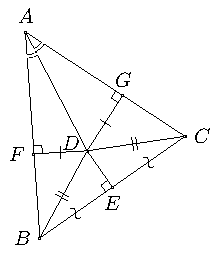
\includegraphics[width=35mm]{img_isocele_ball}
  }
\end{exo}


% ==================================
\section{Utilisation des aires}
% ==================================

\begin{convention}
  On note $\aire (P)$ l'aire d'une figure $P$.
\end{convention}

%-----------------------------------
\begin{exo}

  Soit $T$ un triangle inclus dans un rectangle $R$. Montrer que $\aire(T) \leqslant \frac{1}{2}\aire{R}$.
\end{exo}

%-----------------------------------
\begin{exo} (Théorèmes de Gergonne et de Céva)

  Soient $ABC$ un triangle et $A'$, $B'$, $C'$ trois points de $(BC)$, $(AC)$ et $(AB)$.
  \begin{enumerate}
    \item Si $(AA')$, $(BB')$ et $(CC')$ sont concourantes en un point $M$ intérieur au triangle $ABC$, alors on a la relation de Gergonne
    $$
      \frac{MA'}{AA'}+\frac{MB'}{BB'}+\frac{MC'}{CC'}=1.
    $$
    \begin{indication}
      Interpréter les rapports comme des rapports d'aires.
    \end{indication}
    \item Les trois droites $(AA')$, $(BB')$ et $(CC')$ sont concourantes si et seulement si la relation de Céva
      $$
        \frac{\overline{A'B}}{\overline{A'C}}\frac{\overline{B'C}}{\overline{B'A}}\frac{\overline{C'A}}{\overline{C'B}}=-1.
      $$
  \end{enumerate}
\end{exo}

%-----------------------------------
\begin{exo} (Formule de Héron)

  \begin{enumerate}
    \item Montrer que l'aire d'un triangle $ABC$ de côtés de longueurs $a$, $b$ et $c$ et de demi-périmètre $p=\frac{1}{2}{a+b+c}$ est
    $$
      \aire{(ABC)}=\sqrt{p(p-a)(p-b)(p-c)}.
    $$
    \begin{indication}
      Exprimer $\sin^2(\widehat{A})$.
    \end{indication}
    \item En déduire une expression du rayon du cercle inscrit en fonction des longueurs des côtés.
  \end{enumerate}
\end{exo}

%-----------------------------------
\begin{exo} (Partage de trapèze)

  Soit $ABCD$ un trapèze de grande base $CD$ et de petite base $AB$. Construire un point $M$ de $[CD]$ tel que $(AP)$ partage le trapèze en deux parties de même aire.
\end{exo}

%-----------------------------------
\begin{exo} (Rosace)

  Calculer l'aire de la rosace à 6 feuilles construite au compas.
\end{exo}

%-----------------------------------
\begin{exo}

  Deux disques $\Delta_1$ et $\Delta_2$ de même rayon sont tangents extérieurement et tangents à une même droite $\mathcal D$. Calculer l'aire du disque $\Delta$ tangent à la fois à $\Delta_1$, $\Delta_2$ et $\mathcal D$.
\end{exo}

%-----------------------------------
\begin{exo} (Kangourou 2012)

  \sidebyside{.7}{
    Un morceau de papier rectangulaire $ABCD$, de taille $4$ sur $16$, est plié le long de la droite $(MN)$ de sorte que le sommet $C$ coïncide avec le sommet $A$ (voir la figure).\\
    Quelle est l'aire du pentagone $ABMND'$ ?
  }{
    \raisebox{-14mm}[0pt][0pt]{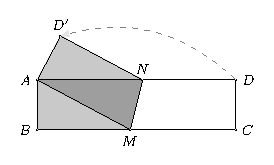
\includegraphics[width=5cm]{img_kangourou2012b}}
  }
\end{exo}

\end{document}
